%!TEX root = ../Report.tex
%********************************************************************
% Appendix
%*******************************************************
% If problems with the headers: get headings in appendix etc. right
%\markboth{\spacedlowsmallcaps{Appendix}}{\spacedlowsmallcaps{Appendix}}

\chapter{Algorithms} \label{chap:app_algo}
\section{Backpropogation}
For a feed forward network\footnote{Other topologies exist with more complex methods for obtaining the weights} with $n_\text{in}$ inputs, $n_\text{hidden}$ hidden units and $n_\text{out}$ output units the back-progogation algorithm works as follows
\begin{enumerate}
\item Initialize network with random weights
\item Repeat until algorithm terminates
\item 
\begin{itemize}
\item $\forall (\vec{x},\vec{t}) \in \text{training examples}$ do
\item 
\begin{enumerate}
\item Input instance $\vec{x}$ to network and compute $o_u\ \forall\ u\ \in \text{network}$
\item For each network output unit $k$ calculate error term\\
$\delta_k \leftarrow o_k (1-o_k)(t_k - o_k)$
\item For each hidden unit $h$ calculate the error term $\delta_h$\\
$\delta_h \leftarrow o_h (1- o_h) \sum_{k \in \text{outputs}} w_{kh}\delta_k$
\item Update each network weight $w_{ji}$\\
$w_{ji} \leftarrow w_{ji} + \eta \delta_j x_{ji}$
\end{enumerate}
\end{itemize}
\end{enumerate}
The complete derivation of the back-propogation algorithm for feed forward artificial neural networks can be found in Mitchell (2007) \cite{Mitchell1997}

\chapter{Platform Specifications}
\begin{table}[h!]
  \centering
  \caption{System specifications}
    \begin{tabular}{l|l}
    \toprule
    Operating System & Windows 8.1 \\
    Memory & 8GB 1333Mhz DDR3 \\
    CPU   & AMD X3 450 3.2GHZ 4 cores \\
    \bottomrule
    \end{tabular}%
  \label{tab:systemspecs}%
\end{table}%

\begin{table}[htbp]
  \centering
  \caption{Development specifications}
    \begin{tabular}{l|l}
    \toprule
    Language & C\# \\
    IDE   & Visual Studio 2015 Community \\
    .NET version & 4.5 \\
    \bottomrule
    \end{tabular}%
  \label{tab:languagespecs}%
\end{table}%


All tests were run with the specifications as given in table \ref{tab:systemspecs}. The development environment specifications are given in figure \ref{tab:languagespecs}.


\chapter{Source Code}
Listed here is the framework used to generate the results mentioned in this project.
\graffito{Code used to algorithmically compose music}

\section{DotNetMusic}
DotNetMusic contains the core music/\ac{MIDI} functionality and includes:
\begin{itemize}
\item Reading and Writing to \ac{MIDI} files using NAudio
\item Core data structures for music representation
\item Core playback functionality
\item \ac{WPF} control for displaying notes on a music sheet
\item Saving and loading of core music data structures using Google protocol buffers
\end{itemize}
DotNetMusic can be found at \href{https://github.com/stefan-j/DotNetMusic}{github.com/stefan-j/DotNetMusic}

\section{DotNetLearn}
Some additional machine learning implementation and useful math features.
\begin{itemize}
\item Implementation of Markov Model
\item Codification of data
\item Other statistical features
\end{itemize}
DotNetLearn can be found at \href{https://github.com/stefan-j/DotNetLearn}{github.com/stefan-j/DotNetLearn}

\section{GeneticMIDI}
GeneticMIDI contains the core functionality for algorithmically generating music.
\begin{itemize}
\item Generators for producing music algorithmically using Markov Models, Markov Chains, Neural Networks.
\item Genetic Algorithms (\ac{GP} tree structures)
\item Fitness functions for Genetic Algorithms including \ac{NCD}, Cosine Similarity (and frequency metrics)
\item Random generation of notes
\item The developed front-end visualizer application for producing music in a user-friendly manner
\end{itemize}

Libraries used include:
\begin{itemize}
\item A-Forge - For the neural networks and evolution of \acp{GA}.
\item Accord - For the \ac{HMM} and neural network training.
\item NAudio - For reading, writing and playing of \ac{MIDI} data. 
\item IKVM - For the \ac{LTSM} network.
\item Proto.Net - .Net implementation of Google protocol buffers for saving of data structures
\end{itemize}

GeneticMIDI can be found at \href{https://github.com/stefan-j/GeneticMIDI}{github.com/stefan-j/GeneticMIDI}

\chapter{Planning}

\graffito{Project breakdown and schedule}


\section{Work Breakdown Structure}
\begin{figure}
\centerline{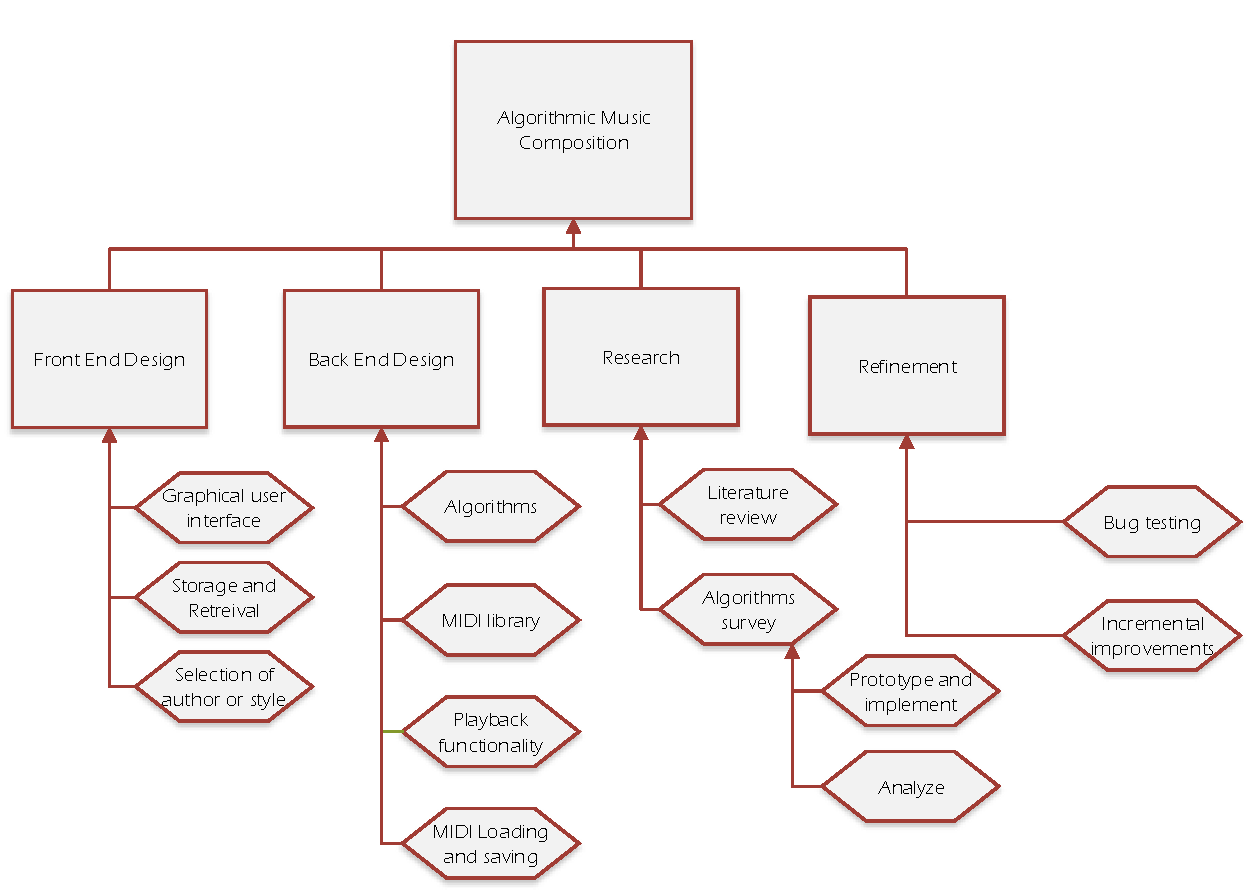
\includegraphics[width=400px]{../images/wbs.pdf}}
\caption{Figure of the work breakdown structure}
\label{ims:sdp}
\end{figure}

Figure \ref{ims:sdp} indicates the work breakdown structure of the project. 
The front end design refers to the user interface and the interaction between the user and the application (IF 1.0).

The back end design refers to the logic of the application and this includes reading the audio files, generating new music and playing music.

Research will be carried out in order to determine the algorithms to be used for algorithmically generating music and to find a suitable framework for developing the software (considering audio playback and similar factors)

Since there are a variety of algorithms, prototyping will be employed to test which algorithms are feasible by means of a trade-off study.

The work breakdown structure allows focus on critical elements of the project and their relation to the whole. This allows us to focus on discrete tasks that are realistic and achievable and keeps the project on track.


\section{Schedule}
% Table generated by Excel2LaTeX from sheet 'Sheet1'
\begin{table}[htbp]
  \centering
  \caption{Schedule for activities}
    \begin{tabular}{lrrr}
    \toprule
    Task Name & Duration & Start & Finish \\
    \midrule
    Algorithms and strategy research & 64 days & Thu 15/01/01 & Tue 15/03/31 \\
    Prototyping of algorithms & 23 days & Tue 15/03/31 & Thu 15/04/30 \\
    Survey and trade-off study & 12 days & Thu 15/04/30 & Fri 15/05/15 \\
    Collection of MIDI samples & 72 days & Fri 15/02/20 & Mon 15/06/01 \\
    Back end framework development & 66 days & Wed 15/04/15 & Wed 15/07/15 \\
    Front end design & 23 days & Wed 15/07/01 & Fri 15/07/31 \\
    Incremental development and testing & 22 days & Fri 15/07/31 & Mon 15/08/31 \\
    Refinement & 31 days & Mon 15/08/31 & Sat 15/10/10 \\
    Milestone 1 & 11 days & Wed 15/02/04 & Wed 15/02/18 \\
    Milestone 2 & 14 days & Sun 15/03/01 & Wed 15/03/18 \\
    Milestone 3 & 11 days & Wed 15/04/01 & Wed 15/04/15 \\
    Milestone 4 & 11 days & Wed 15/05/20 & Wed 15/06/03 \\
    Milestone 5 & 11 days & Wed 15/06/10 & Wed 15/06/24 \\
    Milestone 6 & 10 days & Thu 15/07/02 & Wed 15/07/15 \\
    Milestone 7 & 10 days & Sat 15/08/01 & Thu 15/08/13 \\
    Milestone 8 & 10 days & Thu 15/09/03 & Wed 15/09/16 \\
    Milestone 9 & 9 days & Fri 15/09/25 & Wed 15/10/07 \\
    Milestone 10 & 11 days & Wed 15/10/07 & Wed 15/10/21 \\
    \bottomrule
    \end{tabular}%
  \label{tab:sched}%
\end{table}%

\begin{figure}
\centerline{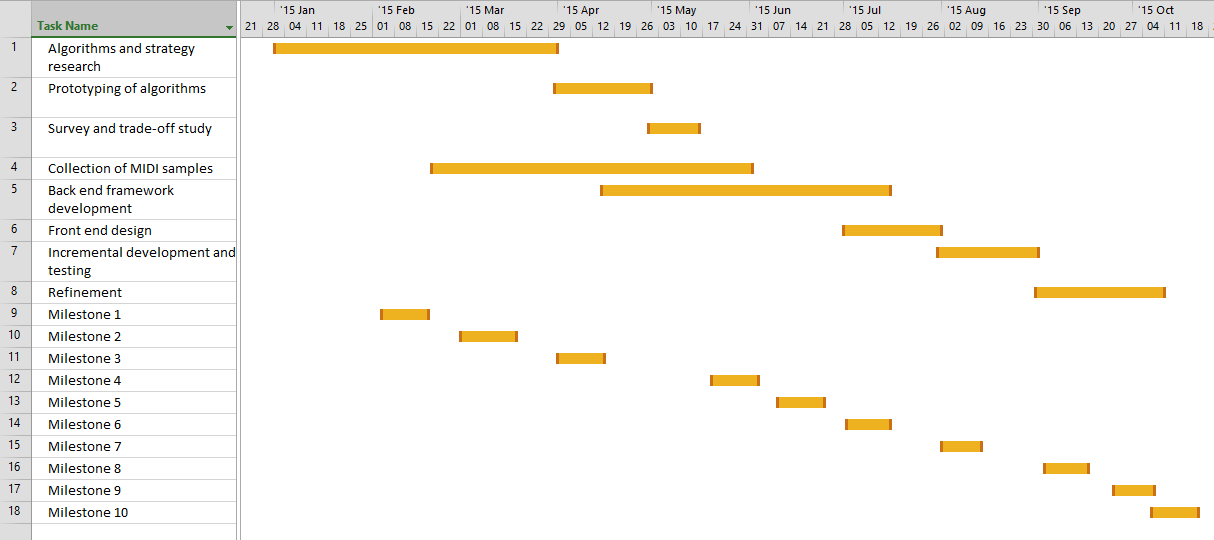
\includegraphics[width=400px]{../images/gantt.png}}
\caption{Gantt chart of project schedule}
\label{ims:gantt}
\end{figure}

In order to successfully complete the project the following tasks must be executed:
\begin{enumerate}
\item Researching machine learning algorithms for music composition
\item Prototyping the algorithms in order to find a feasible subset
\item Collecting a library of audio files to be used as input for machine learning algorithms
\item Developing the required back end components for the software
\item Developing a user interface and designing the interaction components
\item Testing the application, fixing bugs and adding features until the specifications are met 
\end{enumerate}
Table \ref{tab:sched} indicates the estimated length of these activities and the estimated time of completion. Figure \ref{ims:gantt} is a visual representation of the schedule using bar charts.

\section{Budget}
Since the project is a software application no external components will be required. The application will run on a platform that is capable of storing audio files and playing back sound.

Some unplanned costs that might arise include:
\begin{itemize}
\item Internet costs
\item Acquisition cost of audio files
\item Obtaining access to a study or article
\item Audio equipment
\end{itemize}
